%% File: chapters/chapter7.tex
%% Author: Y.U.P. (yashparitkar)
%%
%% Description: Driving the UART wrapper from the graphical interface.

\documentclass[../manual.tex]{subfiles}

\begin{document}

\chapter{The Graphical Interface}
\label{ch:gui}

The graphical front end drives the same \texttt{libre\_ila\_uart} build as Chapter~\ref{ch:cli}, through the same session layer, and does the same things: connect, set a trigger, arm, watch, capture, open the result. What it adds is that the trigger is edited per signal, with the portmap's names in front of you, rather than counted out into one long number.

\section{Starting it}
\label{sec:gui_start}

\begin{lstlisting}
./libre_ila.py --gui
\end{lstlisting}

It needs PySide6, which is the only dependency in this project that the command line does not share; Section~\ref{sec:started_hostpkgs} covers installing it, including on distributions that do not package it. Without it the tool exits with status 10 rather than failing at import, so the rest of the driver keeps working on a machine that has no Qt at all.

\texttt{--waveform-viewer} and \texttt{--portmap} mean the same as they do on the command line and are passed straight through. So does \texttt{--device-dir}, and it matters more here: the window reads the same device store as \texttt{--device}, so a core added in one place shows up in the other only while both are pointed at the same directory. The working directory is the right default for a tool run from a shell and the wrong one for a window started from a desktop entry, which is the case \texttt{--device-dir} exists for.

\section{Tabs and connections}
\label{sec:gui_tabs}

One tab per stored device, titled \texttt{CONNECTED ILA<UID>} or \texttt{DISCONNECTED ILA<UID>}, so the two things worth knowing at a glance are in the tab label. \texttt{+ ADD TAB} introduces a core the same way \texttt{--add-device} does, and it lands in the same store.

A tab owns one session for as long as it lives, so the port is opened once and held rather than reopened per button press. That is the property the whole design rests on: the wrapper is a request and response protocol on a single port, so a connect, several status polls, a trigger read and an arm all have to go through one open port in one order. It is also why the status poll timer stops for the whole readout, since an overlapping poll would desync the wrapper.

\textbf{A tab starts disconnected.} Opening the window opens no ports, which means a window left open does not hold a serial port that something else may want, and a board that is not plugged in yet is not an error at startup. Press \texttt{Connect} when the board is there.

\section{Running a capture}
\label{sec:gui_capture}

The screenshots through this section are the two fake cores of \texttt{tests/python/05\_gui}, rendered with \texttt{make shots}, so every step below can be followed with no hardware attached.

\begin{enumerate}
    \item \textbf{Connect.} A tab opens with its controls idle and its geometry unknown, since nothing has been read yet. Pick the port and baud rate on the right and press \texttt{Connect}. The ILA information box fills in with what the core reports: UID, probe width, buffer depth and sampling frequency. Those four are read out of the core, so they are also the quickest check that you are talking to the core you meant to.
    \begin{figure}[H]
        \centering
        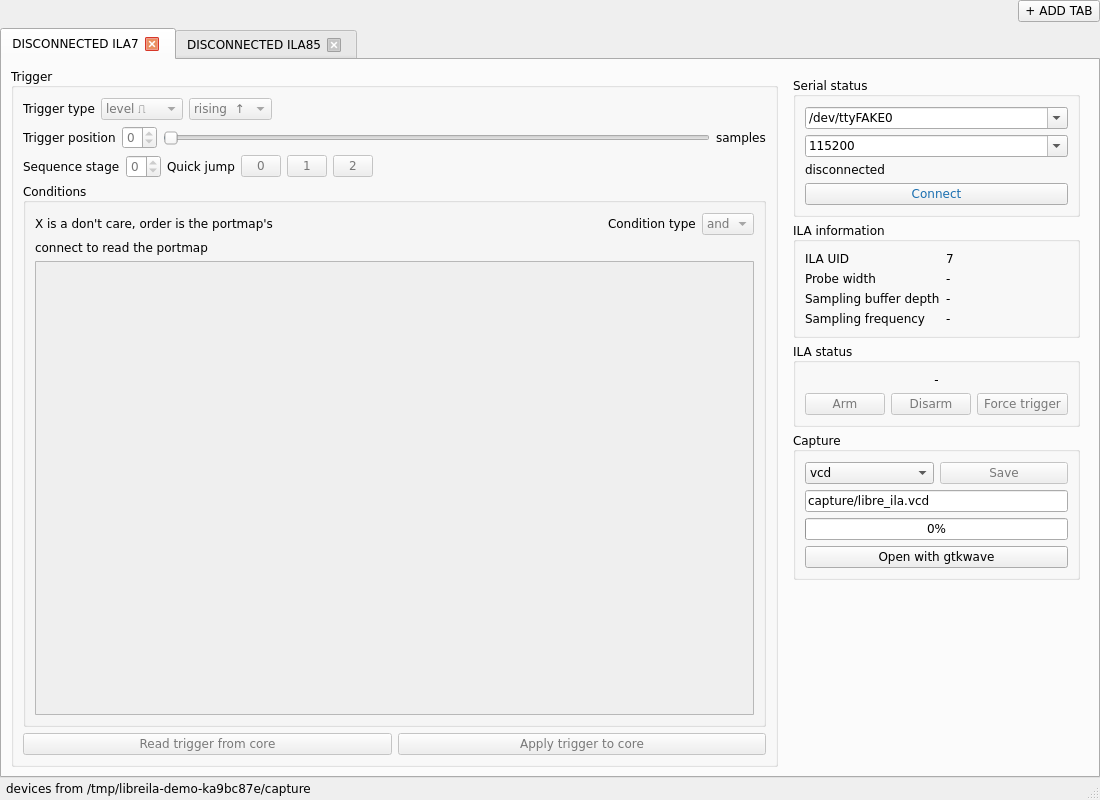
\includegraphics[width=\textwidth]{../images/gui/01-disconnected.png}
        \caption{Two stored cores, both disconnected. The geometry reads \texttt{-} because only the UID is known from the device store.}
        \label{fig:gui_disconnected}
    \end{figure}
    \begin{figure}[H]
        \centering
        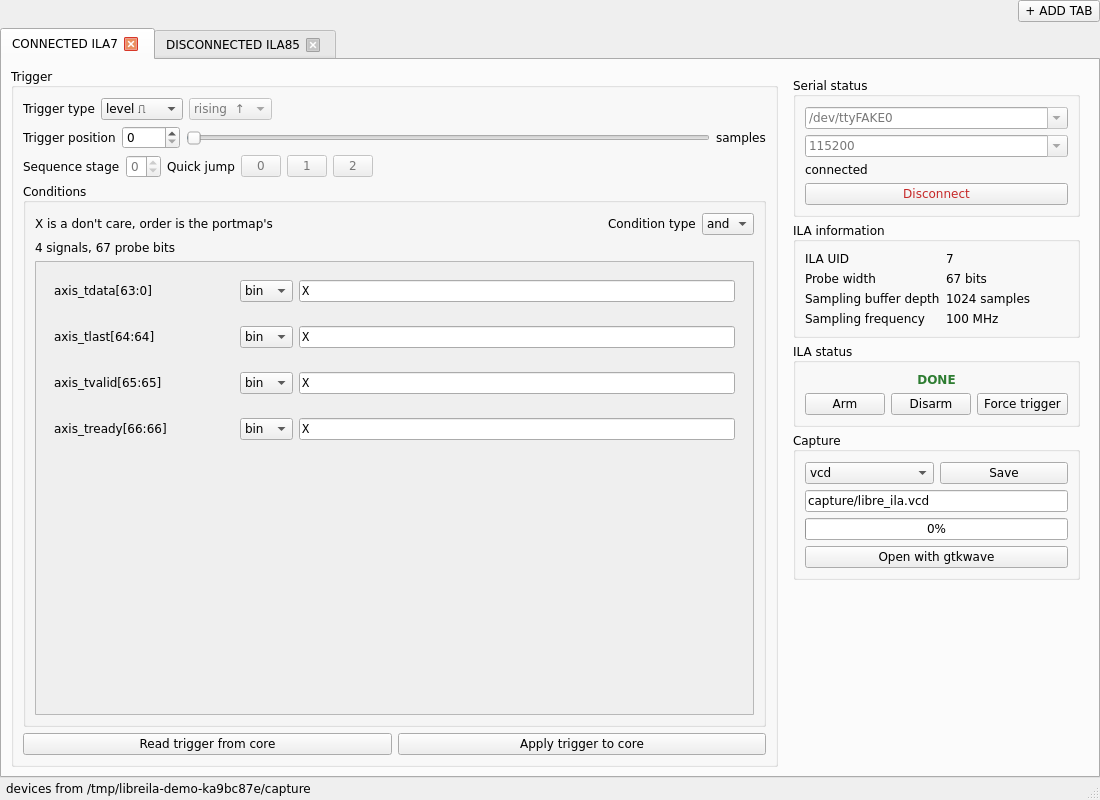
\includegraphics[width=\textwidth]{../images/gui/02-connected.png}
        \caption{The first tab connected. The information box and the conditions table both come from the core.}
        \label{fig:gui_connected}
    \end{figure}
    \item \textbf{Set the trigger.} \texttt{Read trigger from core} loads what the core is currently holding. The conditions table has one row per signal in portmap order, each with a radix and a pattern, where \texttt{X} is a don't care; \texttt{Trigger type} chooses level or edge and, for edge, rising or falling; \texttt{Condition type} chooses whether every signal has to match or any one of them. \texttt{Trigger position} is where in the buffer the trigger sits, in samples.
    \begin{figure}[H]
        \centering
        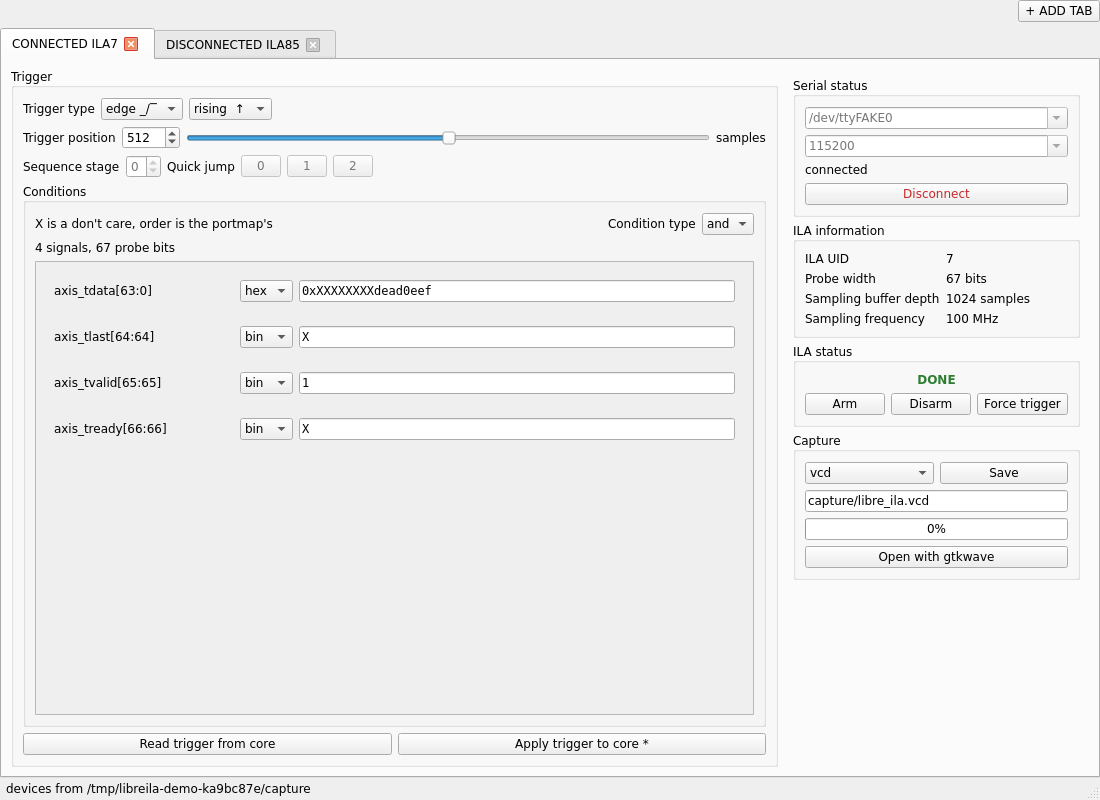
\includegraphics[width=\textwidth]{../images/gui/03-trigger-edited.png}
        \caption{An edited trigger: TDATA matched in hex with the top eight nibbles left as don't cares, TVALID high, the rest ignored, on a rising edge with 512 samples of history. The \texttt{*} on the apply button says the core has not been told yet.}
        \label{fig:gui_edited}
    \end{figure}
    \item \textbf{Apply it.} \texttt{Apply trigger to core} writes the table down as the flat condition and mask pair. Until it is pressed the button carries a \texttt{*}, so an edited table that has not been written is visible rather than assumed.
    \begin{figure}[H]
        \centering
        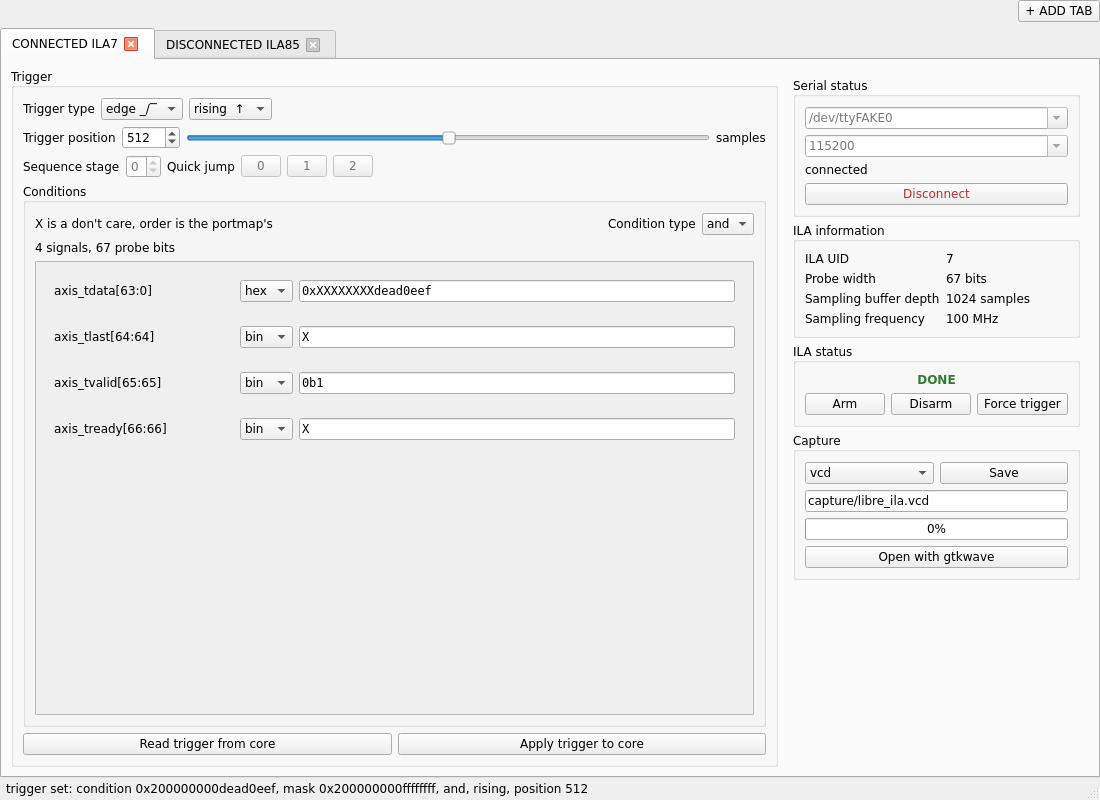
\includegraphics[width=\textwidth]{../images/gui/04-trigger-applied.png}
        \caption{Applied. The status bar shows the flat pair the table became, which is the same pair \texttt{--set-trigger-condition} and \texttt{--set-trigger-mask} take, and the rows now read back as the core holds them.}
        \label{fig:gui_applied}
    \end{figure}
    \item \textbf{Arm.} The status box goes to \texttt{ARMED} with a running timer, so a trigger that never comes looks like a trigger that never comes rather than like a hung window.
    \begin{figure}[H]
        \centering
        
\includegraphics[width=\textwidth]{../images/gui/05-armed.png}
        \caption{Armed and waiting, with the timer counting.}
        \label{fig:gui_armed}
    \end{figure}
    \item \textbf{Force or disarm if needed.} \texttt{Force trigger} fills the buffer from wherever the capture had got to; \texttt{Disarm} returns the core to idle.
    \item \textbf{Capture.} Once the status reads \texttt{DONE}, \texttt{Save} reads the buffer out to the path in the box below it, with the progress bar moving as it comes in. The readout runs off the thread serving the window, which is why the window stays responsive for the seconds it takes.
    \begin{figure}[H]
        \centering
        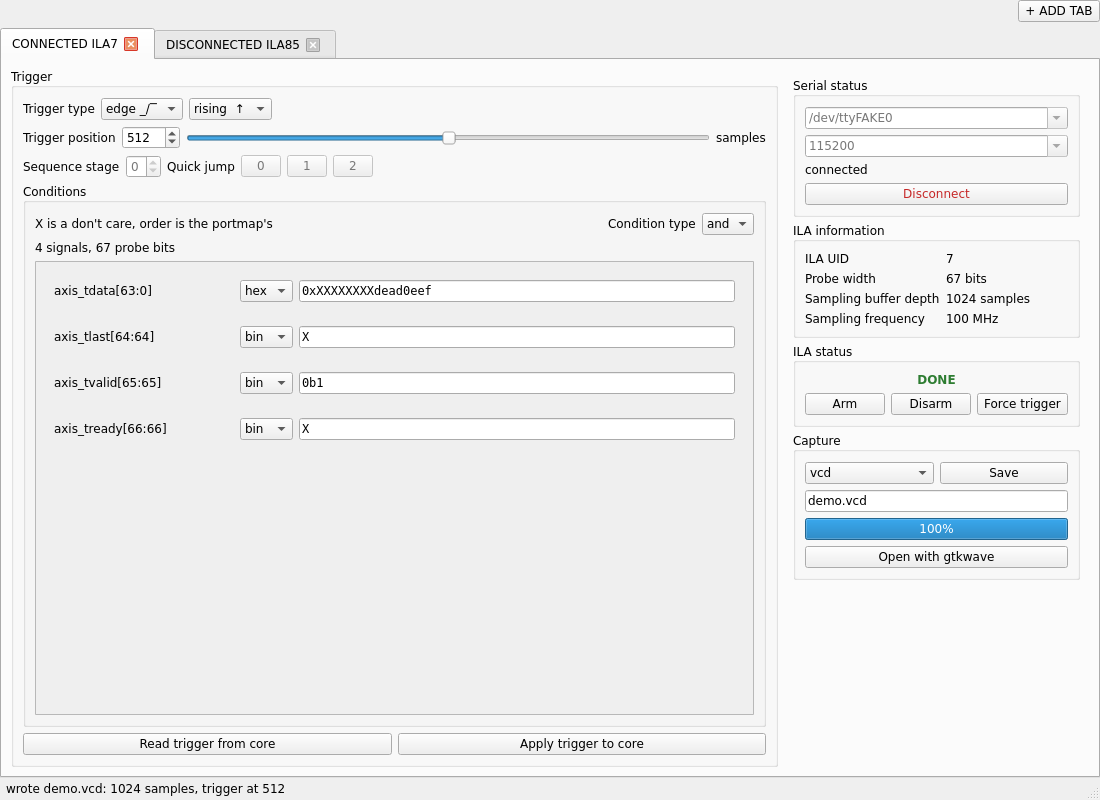
\includegraphics[width=\textwidth]{../images/gui/06-captured.png}
        \caption{Read out and written. The status bar gives the sample count and the row the trigger fired on.}
        \label{fig:gui_captured}
    \end{figure}
    \item \textbf{Open it.} \texttt{Open with gtkwave} launches the waveform viewer on the file just written. Chapter~\ref{ch:reading} covers what is in it.
\end{enumerate}

Figure~\ref{fig:gui_applied} is worth a second look, because it is the whole reason to prefer this front end for setting a trigger. The table above the status bar and the two long numbers in it are the same trigger: the window does the counting that Section~\ref{sec:cli_trigger} has to do by hand.

A refusal from the core, such as disarming an ILA that is already idle, reaches the status bar rather than the event loop. The window survives it and says what happened; nothing about a refused operation closes the connection or loses the tab.

\section{What it does not do yet}
\label{sec:gui_limits}

The \texttt{Sequence stage} and \texttt{Quick jump} controls are visible but disabled, and their tooltip says why: the sequencer needs a core with sequencer registers and this one has none. TRIG\_CFG defines bits 2:0 and nothing else, so there is no register for a stage to live in. They are shown rather than hidden so that the shape of the trigger panel does not change when a core that has them arrives.

The capture format list offers \texttt{vcd} and nothing else so far, which is the same one format the command line writes.

Everything else the command line can do, this can do. If a control you want is missing, the corresponding verb in Chapter~\ref{ch:cli} still exists, and both front ends can be pointed at the same core in turn, since neither keeps any state of its own between operations.

\end{document}
